%! TEX root = ../../master.tex
\lecture[Fun]{Di 17 May 2022}{Missing}
\todo{Content lec09}
\subsection{Integer-optimal solutions in $\LP$ for \emph{some} RHSs}
\begin{align*}
    x(S) &= x(S') + x_{e_k}=x(S')+r(S_k)-r(S_{k-1})\\
    &\leq r(S')+ r(S_k) - r(S_{k-1})\\
    &\leq r(S)
\end{align*}
\begin{note}
    Assume non-degenerate vertices of submodular polyhedron and their permutations. Then there are $n!$ vertices.
\end{note}
Consider permutation. Then $y^*_S$ is dual feasible,  and $y_{S_i}^*=w_i - w_{i-1}$, and $y^*_{S_i} \geq 0$.
Now, $\sum_{S:e\in S} y_S^* \geq w_e$.
This shows for all $e \in E$: $\sum_{S: e \in S} y_S^* = w_e$.

\begin{definition}[Matroid]
    Given a set $\mathcal{J} \subset \{S \subset E\}$. If also
    \begin{enumerate}
        \item $\emptyset \in \mathcal{J}$,
        \item $S \in \mathcal{J}, R \subset S \Rightarrow R \in \mathcal{J}$, and
        \item $R,S \in \mathcal{J}, |R|< |S| \Rightarrow \exists e \in S\setminus R: R+e\in \mathcal{J}$,
    \end{enumerate}
    then $\mathcal{J}$ is a \vocab{matroid}. If only properties (1) and (2) hold, we call it a \vocab{independence system}.
    Property (3) is also called \vocab{extensibility}.
\end{definition}
\begin{definition}[Matroid]
    Let $S \subset E$.
    If \begin{align*}
        r(S) = \max_{I \in \mathcal{J}, I \subset S} |I|
    \end{align*}
    Also $r({e})=0$
\end{definition}
\begin{theorem}
    For all matroids, $r(S)$ is submodular.
\end{theorem}
\begin{proof}
    It suffices to show $R \subset S \subset S+e$, or 
    \begin{align*}
        \underbrace{r(S+e) - r(S)}_{0,1} \leq \underbrace{r(R+e) - r(R)}_{0,1}.
    \end{align*}
    The only bad case is $r(S+e)-r(S)=1$ and $r(R+e)-r(R)=0$.
    Suppose $r(R) = |I_1|, I_1 \in \mathcal{J}, I_1 \subset R$. Set $k = r(S)-r(R) \geq 0$.
    
    From $R \subset S$ it follows from extensibility that (for $K \subset S \setminus R$) there is a $K \subset E$ with $|K|=k$ such that
    \begin{align*}
        r(S)=r(R)+k=|I_1|+|K|,\ I_2=I_1 \cup K, r(S)=|I_2|
    \end{align*}
    Also, from $r(S+e) > r(S)$ it follows from extensibility, that there is $f \in I_2$ such that $I_2+f \in \mathcal{J}$.
    We see that $f=e$, otherwise it follows from $I_2+f \subset S$ that $r(S) > |I_2|$, which is a contradiction.

    Summarizing, we see $I_2+e \in \mathcal{J}$. 
    From property (2) follows that $I_1+e \in \mathcal{J}$.
    Also $I_1 +e \subset R +e$, which implies $r(R+e)=r(R)+1=|I_1|+1$. This contradicts our initial assumption!
\end{proof}
\begin{corollary}
    Greedy works for \emph{any} matroid.
\end{corollary}
\begin{theorem} \label{thm:greedy-ind-is-matroid}
    If Greedy works for all $w$ on an independence system, then it is a matroid.
\end{theorem}
Let $(E,\mathcal{J})$ be an independence system. Then extensibility states,
that additionally all maximal independent subsets of $S$ have the same size, and are thus $\emph{maximum}$.
\begin{example}
    Note the difference of \emph{maximal} and \emph{maximum}! Given following graph:
    \\
    \begin{minipage}{\textwidth}
        \centering
        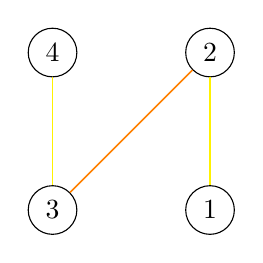
\begin{tikzpicture}
            \begin{scope}[
                    every node/.style={circle, draw},
                    every edge/.style={draw, semithick}
                ]

                \node (1) at (2,0) {$1$};
                \node (2) at (2,2) {$2$};
                \node (3) at (0,0) {$3$};
                \node (4) at (0,2) {$4$};
                
                \path[draw=orange] (2) edge (3);
                \path[draw=yellow] (1) edge (2);
                \path[draw=yellow] (3) edge (4);
            \end{scope}
        \end{tikzpicture}
        % \captionof{figure}{A graph with the spanning tree in black and arc subset $S$ in orange}
    \end{minipage}
    Then the yellow edges form only a maximal matching, while the orange edges a maximum (and maximal) matching.
\end{example}
Define 
\begin{align*}
    \rho(S) = \min \{|I|\mid I \subset S, I \in \mathcal{J}, I\ \text{maximal}\}.        
\end{align*}
Especially, for matroids $\rho(S)=r(S)$.

We want to prove a stronger theorem, though:
\begin{theorem}
    If we apply Greedy to an independence system $(E, \mathcal{J})$, then it holds
    \begin{align*}
        \min_{S \subset E} \frac{\rho(S)}{r(S)}\leq \frac{\text{greedy obj. value}}{\text{optimal obj. value}} \leq 1
    \end{align*}    
    Additionally, the worst case is attainable.
\end{theorem}
\begin{proof}
    Consider $w_{e_1} \geq ... \geq w_{e_n}$ and $S_i\coloneqq\{e_1,...,e_i\}$.
    Let $G \subset E$ be a greedy solution and $G_k \coloneqq G \cap S_k$.
    Let $O \subset E$ be an optimal solution and $O_k \coloneqq G \cap S_k$.

    Consider two cases:
    \begin{itemize}
        \item $e_i \in G$: Then $|G_i| = |G_{i-1}| +1$
        \item $e_i \not \in G$: Then $|G|=|G_{i-1}|$
    \end{itemize}
    Therefore, the greedy objective value is 
    \begin{align*}
        \sum_i (|G_i| - |G_{i-1}|)w_{e_i} &= \sum_i |G_i|(w_{e_i} - w_{e_{i+1}})\\
        &\geq  \sum_i \rho(S_i)(w_{e_i} - w_{e_{i+1}})\\
        &\geq q \sum_i r(S_i)(w_{e_i} - w_{e_{i+1}})\\
        & \geq q \sum_i |O_i|(w_{e_i} - w_{e_{i+1}})\\
        &= q \sum_i (|O_i|-|O_{i-1}|)w_{e_i}\\
        &= q \cdot \ \text{optimal obj. value}
    \end{align*}

    Suppose our $q$ is attained at $S$,
    \begin{align*}
        q = \frac{\rho(S)}{r(S)}.
    \end{align*}
    Therefore there are $I_1,I_2 \subset S$ with $I_1,I_2 \subset \mathcal{J}$
    such that $r(S)=|I_2|$ and $\rho(S)=|I_1|$.

    Choose
    \begin{align*}
        w_e = \begin{cases}
            1, & e \in S\\
            0, & e \not \in S
        \end{cases}.
    \end{align*}
    \todo{graphic}

    Greedy solution will be $I_1$, and optimal solution is $I_2$.
    Therfore $q = \frac{I_1}{I_2}$ as proposed.

\end{proof}
\begin{proof}[Proof for \autoref{thm:greedy-ind-is-matroid}]
    For matroids, $q=1$. Otherwise, $q < 1$.
\end{proof}
\begin{corollary}
    Greedy is a 2-approximation for matching.
\end{corollary}
\begin{example}
    Other matroids are given by:
    \begin{enumerate}
        \item Uniform: $\mathcal{J}=\{S \mid |S| \leq k\}$
        \item Partition: $E$ is partitioned into $P_1,...,P_k$. Then $I \in \mathcal{J}$ iff for all $i$, $|I \cap P_i| \leq 1$.
        
        $G=(N,A),\ P_i = \delta^+(\{i\})$

        $G=(S \cup T,E),\ P_i=\{\delta(\{i\})\}, i \in S$
    \end{enumerate}
\end{example}
\begin{example}
    Independence systems, that are \emph{not} matroids, are for example:
    \begin{enumerate}
        \item Bipartite matching
        \item Branching: $G=(N,A)$, $B \subseteq A$ branching if acyclic, for all $i$, $\delta^- \leq 1$
    \end{enumerate}
\end{example}